\section{Evaluation of Model}
In this section we will evaluate our UPPAAL model on different criteria. First we will evaluate how well our model is capable of emulating reality. This is done by comparing the time it takes for a real life factory configuration to produce sequences of items to the time predicted by our model. Furthermore we will also evaluate how well our optimisations of the model fare. This is done by seeing how the state space and search time for fastest traces increase as we increase the complexity of the model.

\subsection{The Model Compared to Reality}
For comparing our model to reality we used the Festo CP-Factory available at Aalborg University. The current configuration of the CP-Factory when we did this evaluation was a factory that emulates the assembly of mobile phones. We split this configuration up into distinct modules, that could perform specific kinds of work. The configuration that we used for our comparison can be seen in \cref{fig:cp-setup}.

\begin{figure}[h]
\centering
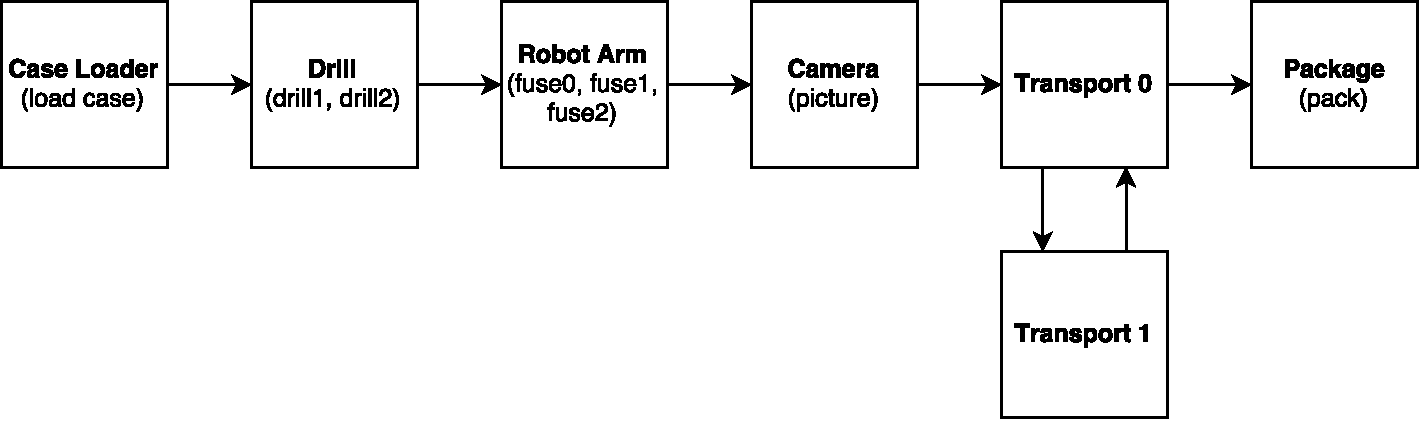
\includegraphics[width=\textwidth]{cp-setup.pdf}
\caption{Graphical representation of the CP-Factory configuration at Aalborg University}
\label{fig:cp-setup}
\end{figure}

After having identified the different modules and the kinds of work they could perform, we seperately ordered single items of three different recipes and timed the travel time between modules, the time it took a module to perform a certain work upon an item and the total time it took for the factory to process the item. The recipes for these items can be seen in \cref{fig:cp-recipes} and the timings can be seen in \cref{tab:cp-time}. This is done so that we can input the time values for how long it takes to travel and work on modules into our UPPAAL model. We can then verify if our models total time is equivalent to the measured total time.

\begin{figure}[h]
\centering
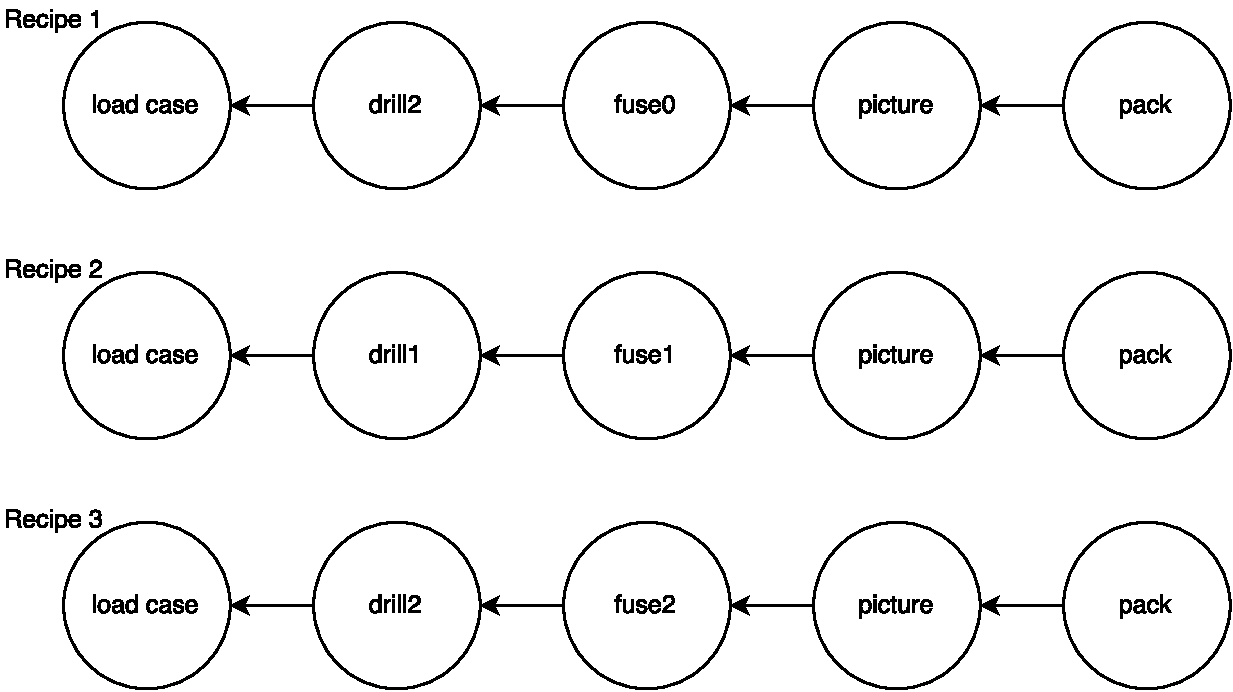
\includegraphics[width=0.5\textwidth]{cp-recipes.pdf}
\caption{Dependency graphs representing the three recipes the CP-Factory could produce}
\label{fig:cp-recipes}
\end{figure}

\begin{table}[]
\centering
\begin{tabular}{ccccc}
\multicolumn{1}{l}{} & \multicolumn{1}{l}{PLACE HOLDER} & \multicolumn{1}{l}{TABLE} & \multicolumn{1}{l}{PLACE} & \multicolumn{1}{l}{HOLDER} \\
recipe 1             & 69                               & 69                        & 69                        & 69                         \\
recipe 2             & 69                               & 69                        & 69                        & 69                         \\
recipe 3             & 69                               & 69                        & 69                        & 69                        
\end{tabular}
\caption{Table showing the time it took for transport through and do different kinds of work on modules. Times are in milliseconds}
\label{tab:cp-time}
\end{table}

We furthermore also did a more complicated order of items, where we wanted one item of each recipe to be produced simultaneously. This is done to verify that our model can also handle working on more than one item at a time. A comparison of our models predictions and the actual times measured can be seen in \cref{tab:cp-result}.

\begin{table}[htb]
\centering
\begin{tabular}{|l|l|l|l|}
\hline
{\ul \textbf{Order Name}} & {\ul \textbf{Actual}} & {\ul \textbf{Simulated}} & {\ul \textbf{Difference}} \\ \hline
\textbf{SingleNoFuse}     & 144.8                 & 144.9                    & 0.1                       \\ \hline
\textbf{SingleLeftFuse}   & 156.5                 & 156.6                    & 0.1                       \\ \hline
\textbf{SingleBothFuse}   & 171.6                 & 171.7                    & 0.1                       \\ \hline
\textbf{AllTypes}         & 305                   & 311                      & 6                         \\ \hline
\end{tabular}
    \caption{Comparison of actual and simulated times. Time is in milliseconds.}
    \label{tab:cp-results}
\end{table}

As seen in \cref{tab:cp-result}, our model accuratly emulates reality to a margin of PLACEHOLDER. It is however importen to keep in mind that the the comparison was done upon a relatively simple and linear system. So we can not be certain that our model would fare as well as it did for this configuration on a more complex configuration. This way of verifying if the model accuratly emulates reality also only work if the items ordered on the real systems a scheduled in a optimal way. As UPPAAL will generate the fastest trace. There are also certain behavious that a factory could have, such as independent queues for items in work and items who want to travel through, that we have not implemented in our model. Adding our removing such behaviours could change the outcome of this evalutation. We however feel confident that our model is capable of accurately mimic the most common modular factories.

 




\subsection{The Complexity of the Model}

It's super fast with a lot of VROOM!
:-) \todo{Vis noget om hvordan vi instantierer og forespørger på systemet}